\documentclass[a4paper, 12pt]{article}
\usepackage{fontspec}
\setlength{\oddsidemargin}{5mm}			% Remove 'twosided' indentation
\setlength{\evensidemargin}{5mm}
\usepackage{fancyhdr}
\usepackage{setspace}
\usepackage{parskip}
\usepackage[hidelinks]{hyperref}
\usepackage[english]{babel}
\usepackage[margin=1.2in]{geometry}
\usepackage{graphicx}

\begin{document}

\begin{titlepage}

% defines new rule for horizoontal lines & thickness
 \newcommand{\HRule}{\rule{\linewidth}{0.5mm}}
 
 \center % center everything
 
 \textsc{\LARGE Loughborough University}\\[1.5cm]
 
 \textsc{\Large COP500}\\[0.5cm]
 
 \textsc{\large Research Methods}\\[0.5cm]
 
\HRule\\[0.4cm]

 {\huge Simultaneous Localisation and Mapping for Driverless Vehicles}\\[0.4cm]

\HRule\\[1.5cm]

\begin{minipage}{0.4\textwidth}
 \begin{center}
   \large
   \textit{Author}: \textsc{Ekow Mensah (B717426)}
 \end{center}
 \end{minipage}

\vfill\vfill


\includegraphics[width=0.7\textwidth]{logo.png}\\[1cm]

\vfill\vfill\vfill
{\large\today}

 
\end{titlepage}
 
\newpage

\tableofcontents{}

\newpage

\section{Introduction}

\onehalfspacing

\subsection{Overview of SLAM}
Wang et al (2011) explain simultaneous localisation and mapping (SLAM) as the process by which an autonomous vehicle constructs a model of its world while concurrently estimating its location within its environment. Originally pioneered by Smith and Cheeseman (1986), SLAM has been a widely researched area by academics in the robotics community for the past two decades because, SLAM enables a robot to localise itself within its environment without prior knowledge of the environment. This is an essential requirement for autonomous robot navigation. Thrun and Leonard (2008) describe the SLAM problem as follows. A mobile robot explores an unknown environment relative to its starting location. Although motion of the robot is unknown, the coordinates of the starting location are maintained. As it the robot explores the environment, the robot uses its sensors to gather information about its environment. SLAM applications are concerned with other aspects such as mapping, sensing, loop closure, kinetics modelling etc. With driverless vehicles specifically, SLAM for autonomous vehicles specifically can be broken down into 4 sub categories. These are:

(Ros et al, 2012)
\begin{itemize}
 \item{Global planning: path computation and goal selection}
 \item{Local motion planning: lateral movement, velocity control and steering control}
 \item{Obstacle Avoidance: road detection, object detection, etc.}
 \item{Traffic Law Enforcement and Engineering: road sign detection and recognition}
\end{itemize}

\parskip 0.2in
Global path planning involves finding a sequence of actions that is required of the robot in a specific location while the robot resides in established point in the environment (Samadi and Othman, 2013). Additionally, Buniyamin et al (2011) define local path planning as online (real-time) avoidance of obstacles using information obtained from sensors concerning exigency measures which influence the safe navigation of the autonomous vehicle. Obstacle avoidance involves the use of sensors such as stereo cameras, light detection and ranging sensors (LiDARS), sound detection and ranging (SONAR) sensors etc., to perceive nearby objects and to distinguish between different types of objects including other vehicles (bikes, trucks), fences and pedestrians in order to prevent collisions and accidents with these objects. Traffic engineering in this context refers to the development of algorithms capable of detecting and recognising road signs and the development of a robot control architecture with the ability to accurately perform actions in accordance with the highway code. 

\subsection{Why SLAM}
According to Durrant-White and Bailey (2006), SLAM has been implemented for both indoor and outdoor applications and has been solved theoretically, conceptually and practically where the environment is static, limited in size and structured, nonetheless, mapping environments which are dynamic and large still poses some challenges (Thrun and Leonard, 2008). Furthermore, new approaches to SLAM require further research in terms of accurately determining the position of the robot in its environment (Evers, 2018).  Therefore, there is a need to review both past and current literature in order to know how to improve existing algorithms and techniques to propose novel approaches to solve existing problems.

\newpage

\section{Research Diagram}

\hspace*{-2cm}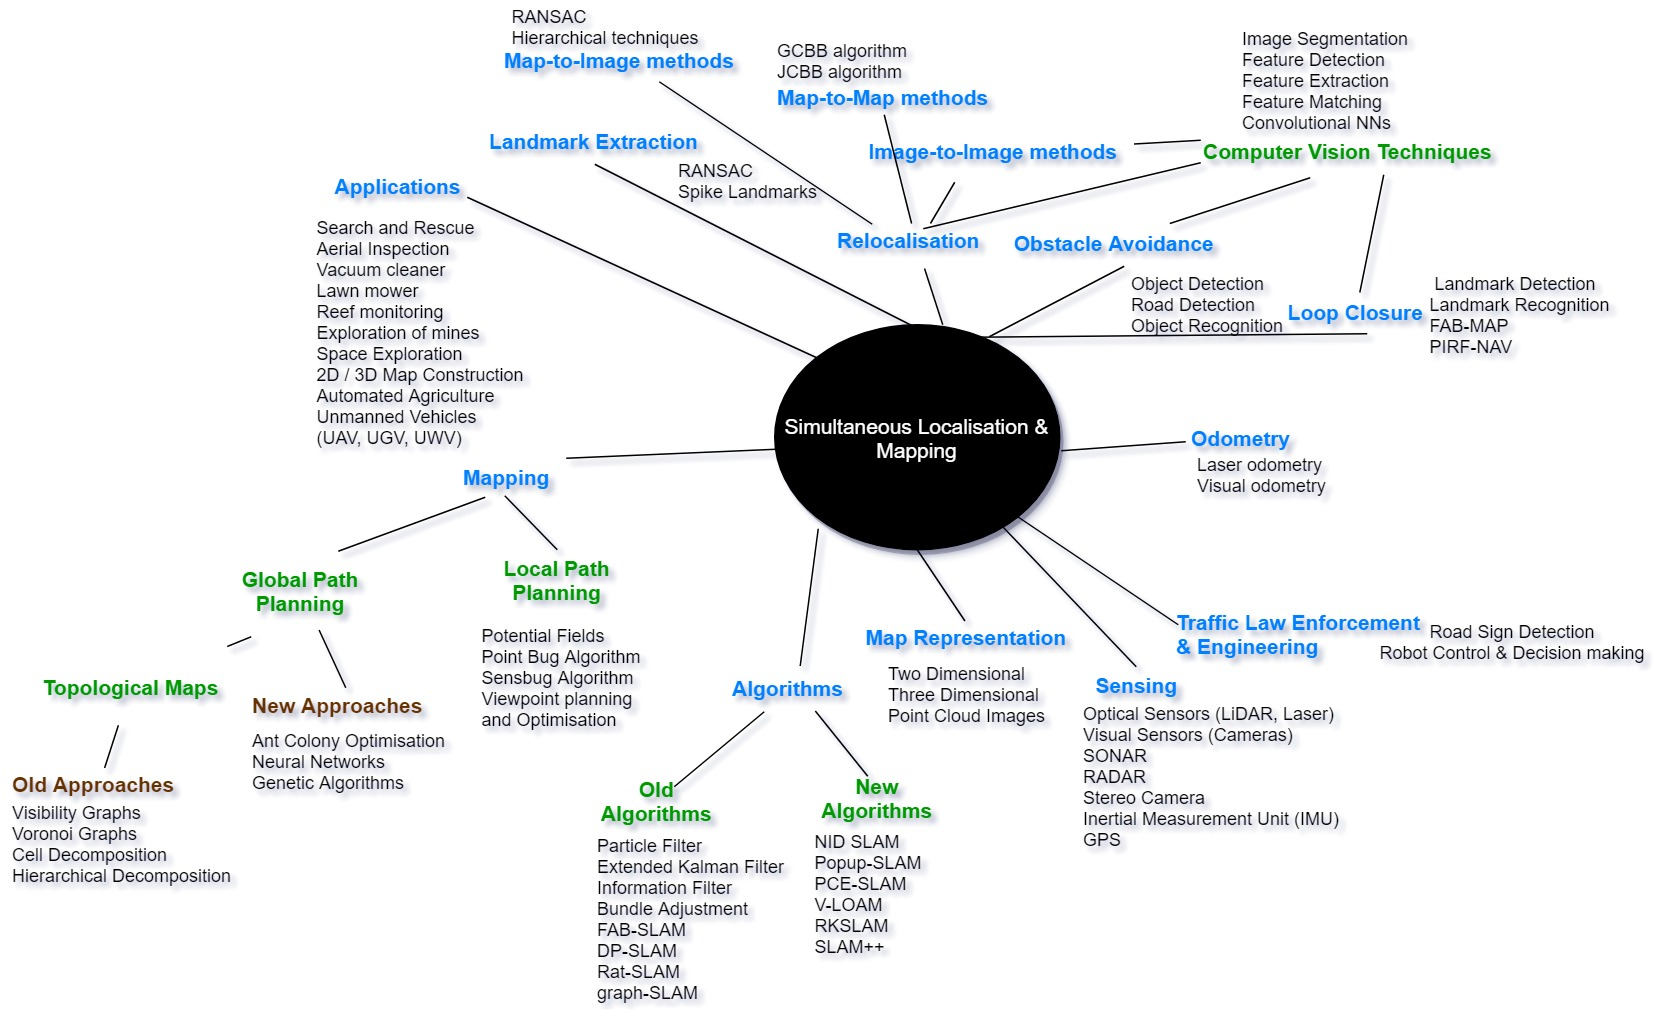
\includegraphics[width=1.3\textwidth, height= 1.1\textwidth]{rdiagram.jpg}\\[1cm]

\newpage 
\section{ Explanation of Research Diagram }
The research diagram in section 2 presents the main concepts and ideas pertaining to SLAM including other related disciplines, old approaches and novel approaches to SLAM methodologies and paradigms. Durrant-White and Bailey (2006) are recognised as the originators of the acronym SLAM and present a detailed explanation of the SLAM problem. Additionally, Durrant-White and Bailey introduce solutions to the SLAM problem such as the Extended-Kalman Filter and the particle filter. The proposed solutions only address the SLAM problem in static environments but fail to function in dynamic environments and the SLAM problem requires a solution that functions effectively in varying environmental conditions. This led to the development of other algorithms such as FAB-MAP (Cummings and Newman, 2008), Rat-SLAM (Milford et al, 2004), DP-SLAM (Eliazar and Parr, 2004) etc.

Milford et al (2004) answer the main questions which are, how to build the map of the environment autonomously and how to localise the robot in its environment, nonetheless, it fails to provide a detailed explanation of why Rat-SLAM fails in outdoor environments although a good test method is proposed for validating Rat-SLAM in outdoor environments. Eliazar and Parr (2004) propose an extension of the DP-SLAM algorithm with an in-depth description and explanation of the mapping aspects of the algorithm (i.e. probabilistic mapping, 2D map representation and observation etc.), however the localisation aspects of SLAM are not addressed in enough detail. Eade and Drummond (2008) put forward a method for loop closure for real-time monocular SLAM using a combination of visual SLAM, image-to-image methods and techniques from computer vision (bag of words model). A decent review of related work is provided, moreover, a detailed description of the proposed loop closure and recovery method is presented with results presented as images showing events of loop closure and recovery. The authors acknowledge faults in the proposed solution and suggest a method (probabilistic model for appearance-based loop closure) to reduce the errors obtained in a worst-case scenario.
 
While most of the studies focus on the localisation problem, Cummings and Newman (2008) concentrate on the mapping problem and provide an elaborate explanation on solutions to the mapping problem including loop closure using techniques from other disciplines such as computer vision (Feature detection \& Extraction) These same authors introduce a solution to the calculation of the vehicles position metrically by using topological maps on a global scale (Cummings and Newman, 2010). A succinct review of related literature is provided in addition to contrasts between existing approaches and the proposed approach. Moreover, the ideas and concepts are presented coherently with detailed explanation of the mathematics behind the suggested concepts. In addition, both aspects of SLAM are addressed with sufficient evidence to ascertain arguments made.
 
Zhang and Singh (2015) suggest a framework (v-LOAM) which makes use of a combination of visual odometry (using cameras) and LiDAR odometry to approximate the ego-motion through the generation of three-dimensional point cloud images which can be applied to autonomous vehicles. The authors clearly assess related work within the field pointing out issues current methods in comparison with the proposed technique. Furthermore, a comprehensive description of the proposed method is given along with test results to prove the validity of the suggested method. However, a limitation of this study is that, testing is only done indoors and not outdoors and therefore, there is not enough evidence to prove that the technique will be useful for vehicles operating outdoors. On the other hand, Agrawal et al (2017) propose a real-time PCE-SLAM algorithm with consideration of outdoor conditions using LiDAR data. Gaps in literature tackling problems relating to LiDAR based SLAM are identified. Additionally, the components of the proposed algorithm (motion estimation, feature extraction, feature correspondence etc.), are explained logically with test results of both indoor and outdoor environments as evidence of a working system. More importantly, a gap in the proposed solution (that is, does not account for loop closures) is recognised which helps direct the next stage of research. 

Similar to Cummings and Newman (2008), Pierzchała et al (2018) focus solely on the mapping component of SLAM and introduce the use of graph-SLAM to generate three dimensional maps obtained from laser scans dependent on laser odometry for forest environments using sensors such as IMU, LiDAR, stereo cameras and GPS and an unmanned ground vehicle. The authors provide a relatively detailed introduction on the main ideas and concepts, however, a more detailed review of related work could have been provided. Nevertheless, the methodology and tests and results are described and explained very well with evidence provided in the form of tables and images for the results section. The authors acknowledge the possible research opportunities that have been created due to the results obtained from the project and therefore emphasises the need for more research in SLAM for forest environments.  

\newpage
Path planning is an essential topic which is related to SLAM. This is because, path planning helps with both localisation and mapping in that, it is possible to recognise a specific location or position once it has been visited before. This can be achieved using path planning techniques. Garrido et al (2006) explain the use of Voronoi graphs/diagrams for autonomous robot navigation and fast marching based on sensor information. Although the information provided in the article is relatively detailed with explanations of the main concepts (i.e. fast marching method and Voronoi diagram), there is no review on past or related work. This would have been helpful because, it will shed some light on the depth of research carried out under this topic area and the motivation for the research. Newer approaches to global path planning include artificial neural networks, genetic algorithms and ant colony optimisation as seen in the research diagram above. Chen and Chiu (2015) present an optimal robot path planning system using both genetic algorithms and artificial neural networks. Besides the fact that the main concepts are relatively elaborated, this method only focuses and works on indoor path planning and ignores the potential for the proposed algorithm to be used outdoors. Nonetheless, the proposed approach Furthermore, similar to Garrido et al., a succinct review of related work would help understand the associations between established concepts. 

Most of the challenges pertaining to SLAM for driverless vehicles involve the need to build high definition maps at both a metric and a topological level and  (Bresson et al, 2017). Seif and Hu (2016) explain the need for high definition maps as a requirement for driverless vehicles. 3 main SLAM related problems are stated in the introduction which are the ability of the vehicle to localise itself in the environment with high precision, perform actions based on sensor information obtained from the road and ability of vehicle to drive in accordance with traffic regulations and other vehicles on the road respectively. The authors focus more on the generation of high definition maps and using adhoc networks to enable communication between other vehicles on the road which address the first and third problem, however, no literature is provided or comments were made to address the second problem that was stated. Walcott and Eustice propose a robust LiDAR localisation technique using multi resolution mixture maps for driverless vehicles which considers other related topics such as loop closures, feature extraction. A brief review of related work is provided with citations of the works of prominent authors such as Newman and Thrun. Moreover, a very in-depth discussion of concepts is also provided including experiments and results of the experiments validate the concepts explained. Furthermore, the tests were conducted outdoors in varying weather conditions which is very relevant to driverless cars. 

\section{Conclusion}
In conclusion, literature concerned with SLAM ranging from various years (2004 - 2018) has been reviewed. SLAM has been extensively researched and as a result, there is a wide range of literature available. Most of the literature tend to focus either the localisation aspects or the mapping aspects, although some papers focus on both aspects. Furthermore, a wide range of approaches have been used to solve the SLAM problem which has led to the development of various algorithms with a few mentioned in the research diagram. Also, most of the literature reviewed provide a detailed explanation of the concepts and related theories as well provide results of any experiments or tests carried out. A main finding was that some of the papers only focused on indoor localisation and mapping without considering potential for outdoor localisation and mapping which is more relevant to driverless vehicles. Furthermore, some papers provided further research directions and opportunities to explore. 


\newpage
\section{Reference List}

Agrawal, P., Iqbal, A., Russell, B., Hazrati, M., K., Kashyap, V.,
and Akhbari, F. (2017) \textit{PCE-SLAM: A Real-time Simultaneous Localization and Mapping using LiDAR data}. \textit{2017 IEEE Intelligent Vehicles Symposium (IV)} Redondo Beach, CA, USA, June 11 - 14 2017. California:IEEE pp. 1752 - 1757.

Bresson, G., Alsayed, Z., Yu, L. and Glaser, S. (2017). Simultaneous Localization and Mapping: A Survey of Current Trends in Autonomous Driving. \textit{IEEE Transactions on Intelligent Vehicles}, [online] 2(3), pp.194-220. Available at: \url{https://hal.archives-ouvertes.fr/hal-01615897/file/2017-simultaneous_localization_and_mapping_a_survey_of_current_trends_in_autonomous_driving.pdf} (Accessed: 8th March 2018).

Buniyamin N., Sariff N., Wan Ngah W.A.J., Mohamad Z. (2011) Robot global path planning overview and a variation of ant colony system algorithm, \textit{International Journal Of Mathematics And Computers In Simulation}, [online] 5(1), pp 10-16. Available at: \url{https://pdfs.semanticscholar.org/4c53/70100a2ac53562d13c0ac61466edf1d213ea.pdf} (Accessed: 8th March 2018).   

Chen, Y., W. and Chiu, W., Y. (2015) \textit{Optimal Robot Path Planning System by Using a Neural Network-Based Approach}. Yilan, Taiwan 18-20 Nov. 2015. Yilan:IEEE pp 85-90.

Cummins, M. and Newman, P. (2008). FAB-MAP: Probabilistic Localization and Mapping in the Space of Appearance. \textit{The International Journal of Robotics Research}, [online] 27(6), pp.647-665. Available at: \url{http://journals.sagepub.com/doi/abs/10.1177/0278364908090961} (Accessed: 8th March 2018).

Cummins, M. and Newman, P. (2010). Appearance-only SLAM at large scale with FAB-MAP 2.0. \textit{The International Journal of Robotics Research}, [online] 30(9), pp.1100-1123. Available at: \url{http://journals.sagepub.com/doi/pdf/10.1177/0278364910385483} (Accessed: 8th March 2018).

Durrant-Whyte, H. and Bailey, T. (2006). Simultaneous Localisation and Mapping (SLAM): Part I The Essential Algorithms. [online]. Available at: \url{https://people.eecs.berkeley.edu/~pabbeel/cs287-fa09/readings/Durrant-Whyte_Bailey_SLAM-tutorial-I.pdf} (Accessed: 8th March 2018).

Eade, E. and Drummond, T. (2008) \textit{Unified Loop Closing and Recovery for Real}. [online]. Available at: \url{http://mi.eng.cam.ac.uk/~ee231/bmvc2008.pdf
Time Monocular SLAM} (Accessed 8th: March 2018).

Eliazar, A., and Parr, R. (2015) \textit{DP-SLAM 2.0}. \textit{Proceedings. ICRA '04. 2004 IEEE International Conference on Robotics and Automation} New Orleans, LA, USA 26 April - 1 2004. New Orleans:IEEE pp 1314-1320.

Evers, C. and Naylor, P. (2018). Optimized Self-Localization for SLAM in Dynamic Scenes Using Probability Hypothesis Density Filters. \textit{IEEE Transactions on Signal Processing}, [online] 66(4), pp.863-878. Available at: \url{http://ieeexplore.ieee.org/stamp/stamp.jsp?arnumber=8116669&tag=1} (Accessed 8th: March 2018).

Garrido, S., Moreno, L., Abderrahim, M., and Martin, F. (2006) \textit{Path Planning for Mobile Robot Navigation using Voronoi Diagram and Fast Marching}. \textit{Proceedings of the 2006 IEEE/RSJ International Conference on Intelligent Robots and Systems}. Beijing, China October 9 - 15, 2006. Beijing:IEEE pp. 2376 - 2381.

Milford, M., Wyeth, G. and Prasser, D. (2004). RatSLAM: a hippocampal model for simultaneous localization and mapping. \textit{IEEE International Conference on Robotics and Automation, 2004. Proceedings. ICRA '04. 2004}. [online] Available at: \url{http://ieeexplore.ieee.org/document/1307183/} (Accessed: 8 March 2018).

Pierzchałaa, M., Giguèreb, P., Astrupa, R. (2018) Mapping forests using an unmanned ground vehicle with 3D LiDAR and graph-SLAM, \textit{Computers and Electronics in Agriculture}, [online] 145 pp 217-225. Available at: \url{https://www.sciencedirect.com/science/article/pii/S0168169917301631} (Accessed: 8th March 2018).

Ros, G., Sappa, A, D., ., Ponsa, D.and Lopez, A., M. (2012) Visual SLAM for Driverless Cars: A Brief Survey, \textit{Proceedings of the 2012 IEEE Intelligent Vehicles Symposium Workshops} [online] pp. 1-6. Available at: \url{http://www.cvc.uab.es/~asappa/publications/C__IEEE_IV_2012_W3.pdf} (Accessed: 7th March 2018)

Samadi, M. and Othman, M. (2013). Global Path Planning for Autonomous Mobile Robot Using Genetic Algorithm. \textit{2013 International Conference on Signal-Image Technology \& Internet-Based Systems}, [online] pp.726 - 729. Available at: \url{http://ieeexplore.ieee.org/document/6727268/} (Accessed 8th: March 2018).

Seif, H. and Hu, X. (2016). Autonomous Driving in the iCity—HD Maps as a Key Challenge of the Automotive Industry. \textit{Engineering}, [online] 2(2), pp.159-162. Available at: \url{https://www.sciencedirect.com/science/article/pii/S2095809916309432} (Accessed: 9th March 2018).

Smith, R. and Cheeseman, P. (1986) On the Representation and Estimation of
Spatial Uncertainty, \textit{The International Journal of Robotics Research},
5(4) pp. 56–68. 

Thrun, S. and Leonard, J., J. (2008) Simultaneous Localization and Mapping. In: Khatib, S. (eds) \textit{Springer Handbook of Robotics}. Springer.

Wang, Z., Huang, S. and Dissanayake, G. (2011) \textit{Simultaneous Localisation and Mapping Exactly Sparse Information Filters}. Singapore: World Scientific Publishing Co. Pte. Ltd.

Zhang, J., and Singh, S. (2015) \textit{Visual-lidar Odometry and Mapping: Low-drift, Robust, and Fast}. \textit{2015 IEEE International Conference on Robotics and Automation (ICRA)} Washington State Convention Center May 26-30. Seattle, Washington IEEE:pp 2173 - 2181.






\end{document}